\documentclass[svgnames, 10pt]{beamer}

\usepackage[utf8]{inputenc}
\usepackage[english]{babel}
\usepackage[L7x]{fontenc}
\usepackage{amsmath}
\usepackage{amssymb}
\usepackage{lmodern}
\usepackage{xcolor}
\usepackage{subfig}

\definecolor{mifcolor}{RGB}{0, 71, 127}
\definecolor{dimgr}{RGB}{105, 105, 105}
\definecolor{sky}{RGB}{0, 191, 255}
\setbeamercolor{alerted text}{fg=red,bg=sky}

\mode<presentation>{
\usetheme{Madrid}
\usecolortheme[named=mifcolor]{structure}
}

\title[Air Pollution in India]{Predicting Air Pollution Levels in Five Major Indian Cities}
\author{Aleksandr Jan Smoliakov \and Danial Yntykbay \and Davide Giuseppe Griffon}
\institute[VU]{Data Science Study Programme\\Faculty of Mathematics and Informatics}
\date{2024}

\begin{document}

\begin{frame}
\titlepage
\end{frame}

\begin{frame}{Table of Contents}
\tableofcontents
\end{frame}

\section{Introduction}

\begin{frame}{Project Overview}
    \begin{itemize}
        \item Background:
            \begin{itemize}
                \item Air pollution ranks among the most pressing global health threats
                \item India faces some of the highest pollution levels globally
                \item Driven by rapid urbanization and economic growth
            \end{itemize}
        \vspace{1em}
        \item Study Objectives:
            \begin{itemize}
                \item Analyze pollution and weather data from five major Indian cities:
                    \begin{itemize}
                        \item Bengaluru, Delhi, Hyderabad, Jaipur, Mumbai
                    \end{itemize}
                \item Develop predictive models using multivariate linear regression
                \item Focus on understanding key meteorological and temporal predictors
            \end{itemize}
    \end{itemize}
    \vfill
 \end{frame}


\begin{frame}{Literature Review}
    \begin{itemize}
        \item Extensive research available:
            \begin{itemize}
                \item Widespread interest among scientists and data analysts
                \item Numerous studies on air pollution
                \item Many also are focused on India due to severe air quality issues
            \end{itemize}
        \item Research gap:
            \begin{itemize}
                \item No existing studies examining these five specific cities together
                \item Unique combination of air quality and weather datasets
            \end{itemize}
        \item Most existing approaches:
            \begin{itemize}
                \item Deep learning / neural network models
                \item Complex machine learning algorithms
            \end{itemize}
        \item Our approach:
            \begin{itemize}
                \item Focus on interpretable linear regression
                \item Emphasis on feature engineering
                \item Independent models for each city and pollutant
            \end{itemize}
    \end{itemize}
\end{frame}

\section{Data Analysis}

\begin{frame}{Data Sources}
    \begin{itemize}
       \item Air Quality Data in India (2015-2020):
           \begin{itemize}
               \item Hourly pollution measurements
               \item Coverage: 27 major Indian cities
               \item Over 700,000 records
           \end{itemize}
       \vspace{0.5em}
       \item Historical Weather Data (2006-2019):
           \begin{itemize}
               \item Over 20 meteorological variables
               \item Coverage: 8 Indian cities
               \item Over 700,000 records
           \end{itemize}
       \vspace{0.5em}
       \item Combined Dataset:
           \begin{itemize}
               \item Time period: January 2015 to December 2019
               \item Five cities with complete data coverage:
                   \begin{itemize}
                       \item Bengaluru, Delhi, Hyderabad, Jaipur, Mumbai
                   \end{itemize}
           \end{itemize}
    \end{itemize}
    \vfill
\end{frame}

\begin{frame}{Preliminary Analysis}
    \begin{itemize}
       \item Correlation between pollutants:
           \begin{itemize}
               \item Most pollutants positively correlated with each other
               \item O\textsubscript{3} shows distinct pattern from other pollutants
           \end{itemize}
       \item Weather correlations:
           \begin{itemize}
               \item Humidity: negative correlation with most pollutants
               \item Wind speed: negative correlation, aids pollutant dispersion
               \item Temperature: positive correlation with O\textsubscript{3}
               \item UV index: positive correlation with O\textsubscript{3}
           \end{itemize}
       \item Temporal patterns:
           \begin{itemize}
               \item Strong seasonal trends observed
               \item Higher pollution in autumn and winter
           \end{itemize}
    \end{itemize}
\end{frame}

\begin{frame}{Preliminary Analysis}
    \vspace{0.5em}
    \begin{center}
        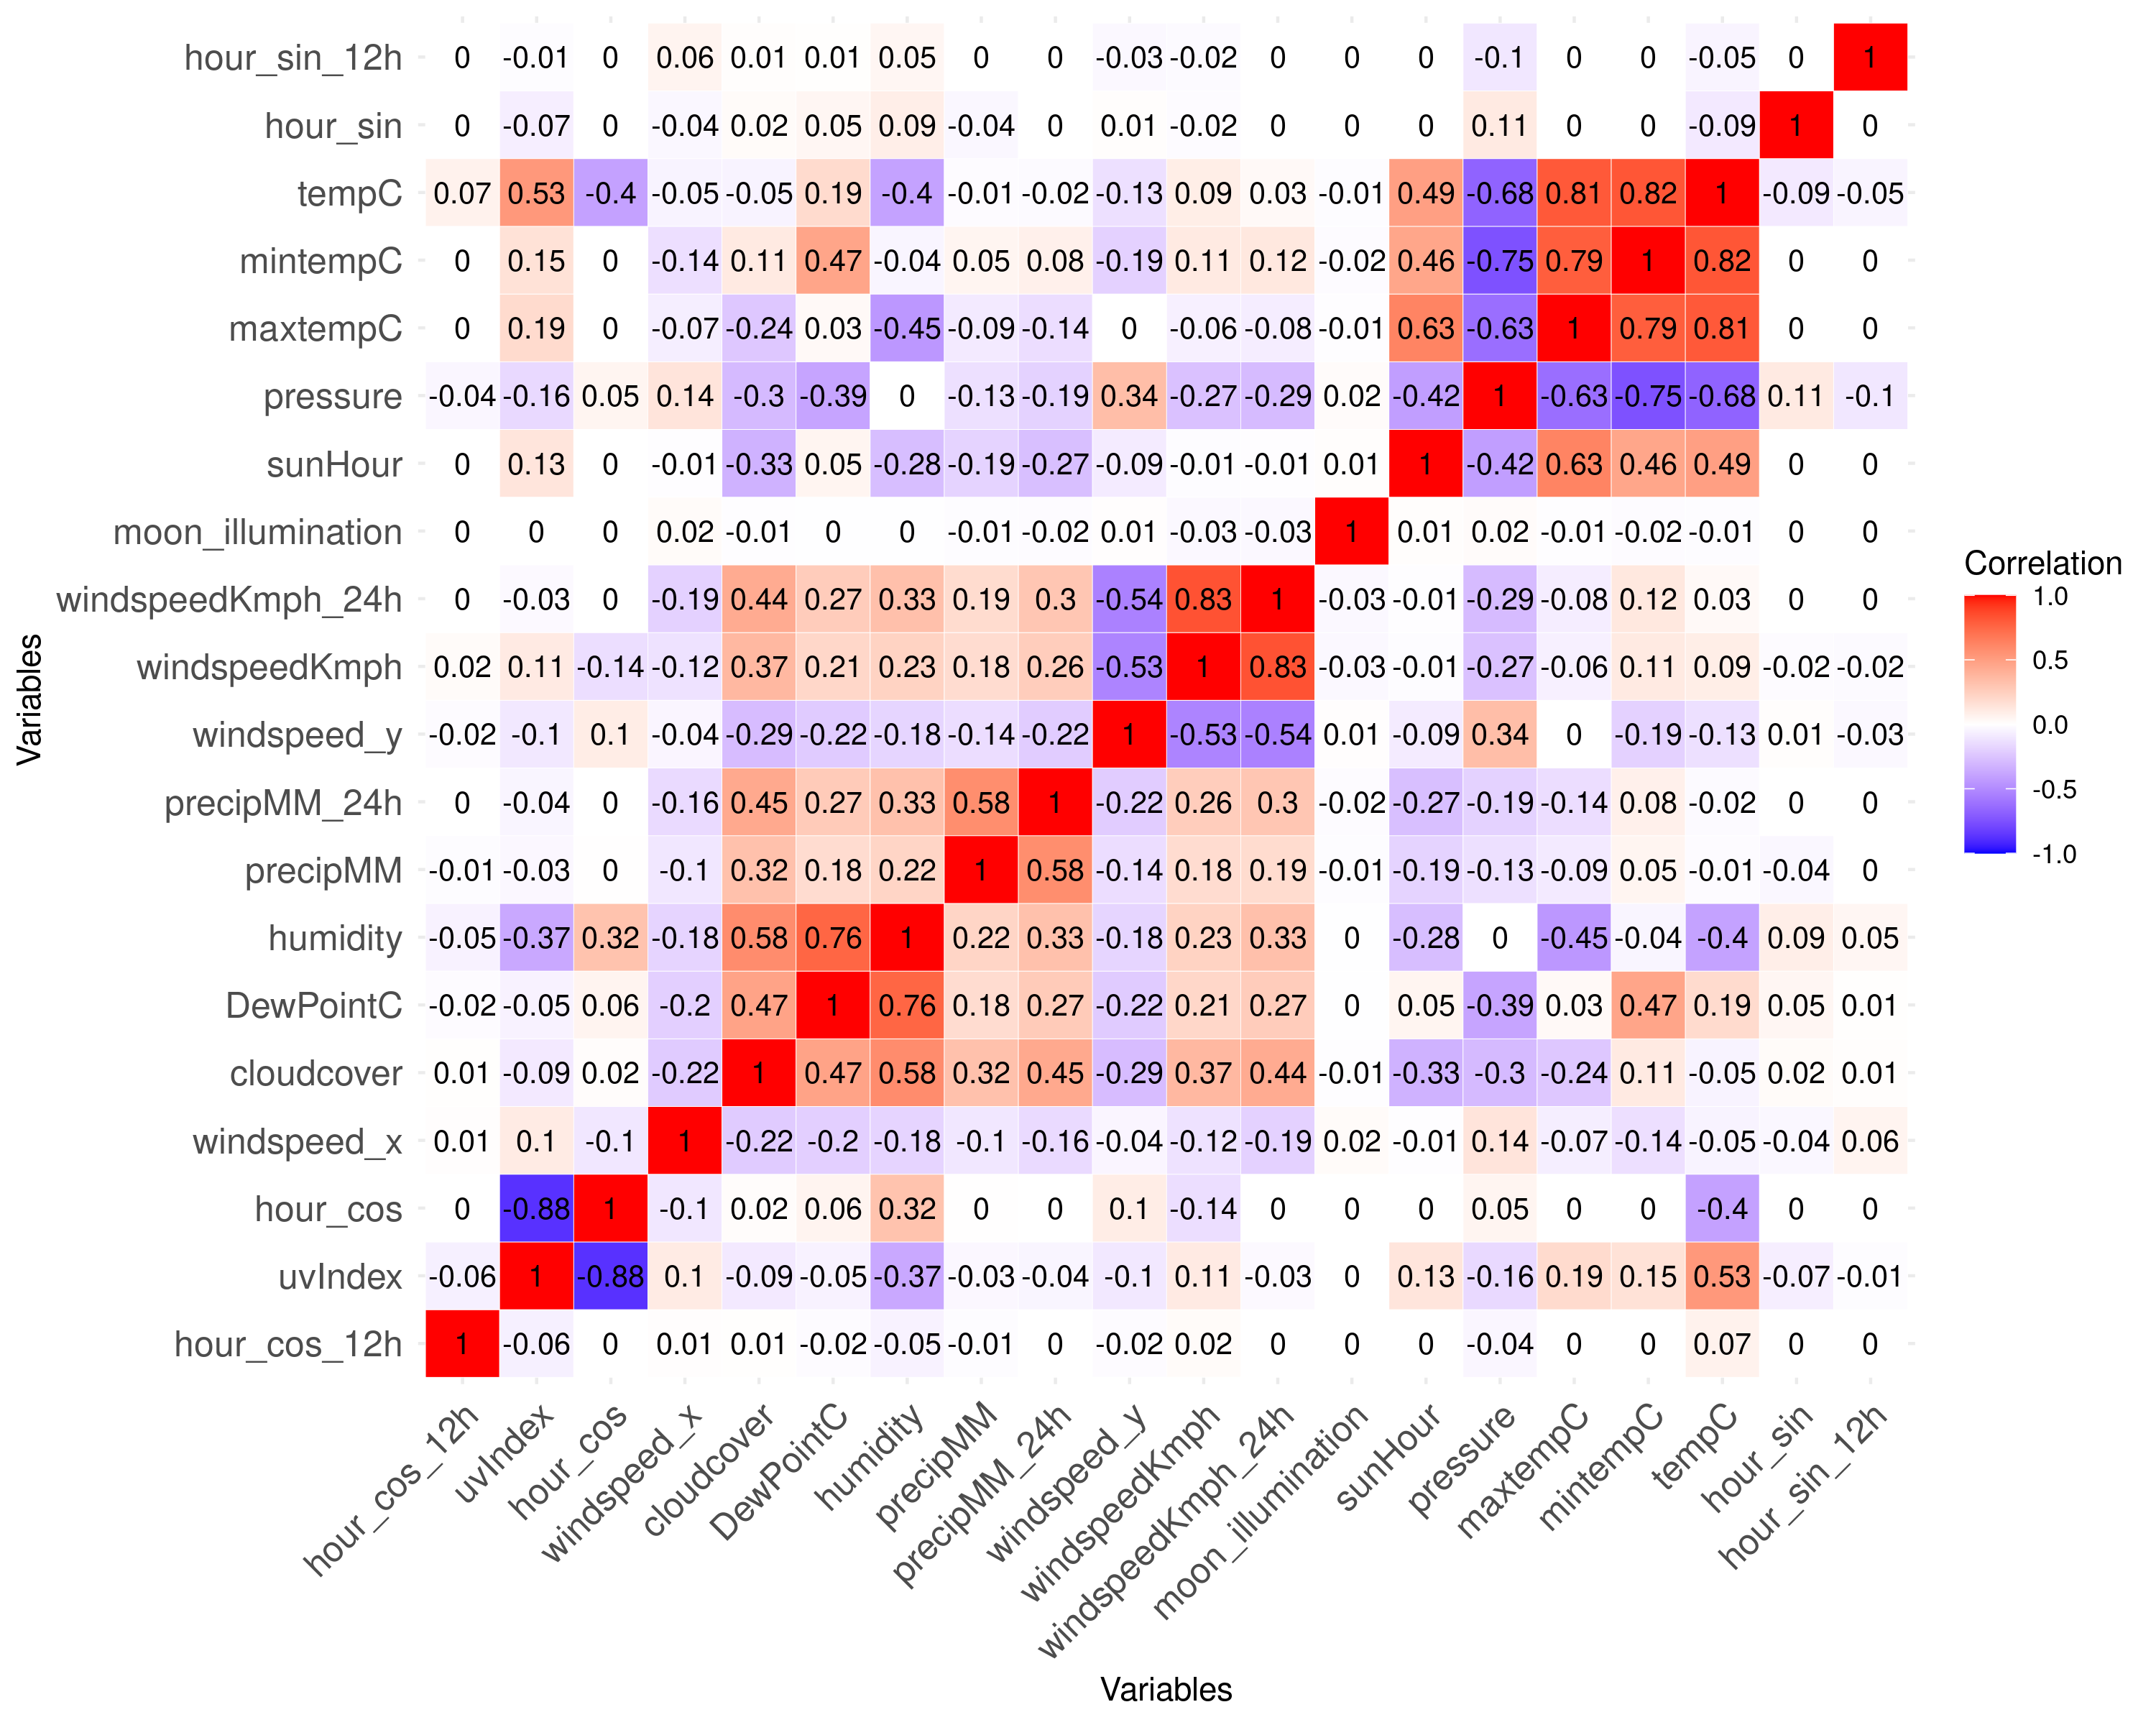
\includegraphics[width=0.8\textwidth]{assets/feature-correlation-matrix-final.png}
    \end{center}
    \vfill
\end{frame}

\begin{frame}{Original Data Distribution}
    \begin{itemize}
        \item Initial analysis revealed strongly right-skewed distributions:
            \begin{itemize}
                \item High frequency of lower values
                \item Long tail extending toward higher concentrations
                \item Pattern consistent across all pollutants and cities
            \end{itemize}
    \end{itemize}
    \vspace{1em}
    \begin{center}
        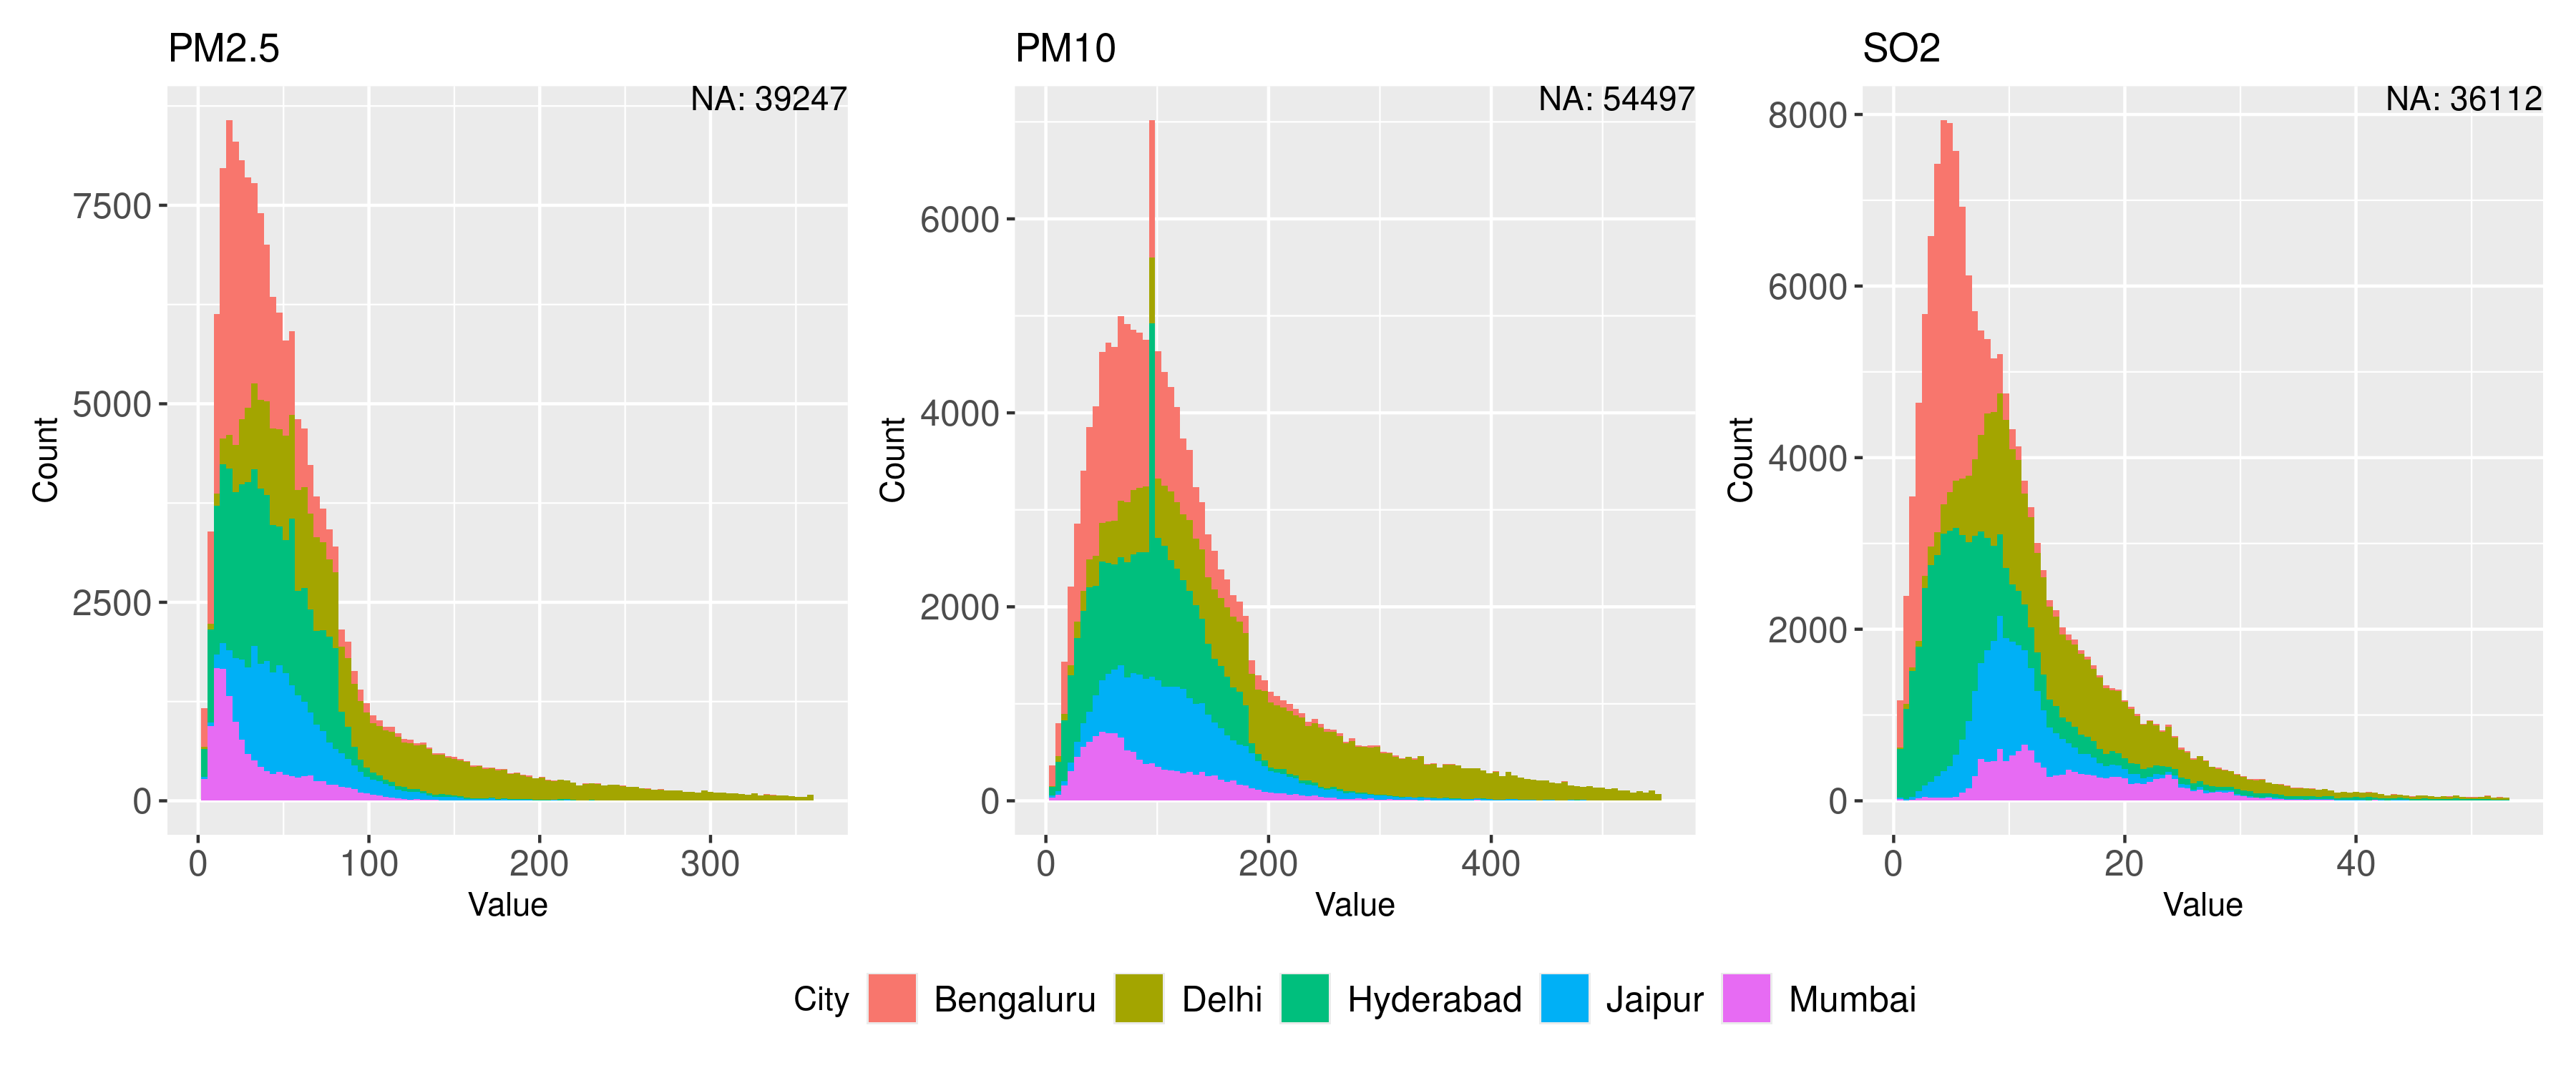
\includegraphics[width=0.7\textwidth]{assets/skewness.png}
    \end{center}
    \vfill
\end{frame}

\begin{frame}{After Log Transformation}
    \begin{itemize}
        \item Applied logarithmic transformation to address skewness:
            \begin{itemize}
                \item Added constant of 1 to handle zero values
                \item Resulted in more normal-like distributions
                \item Data better suited for linear regression
                \item Transformation applied consistently across all pollutants
            \end{itemize}
    \end{itemize}
    \vspace{1em}
    \begin{center}
        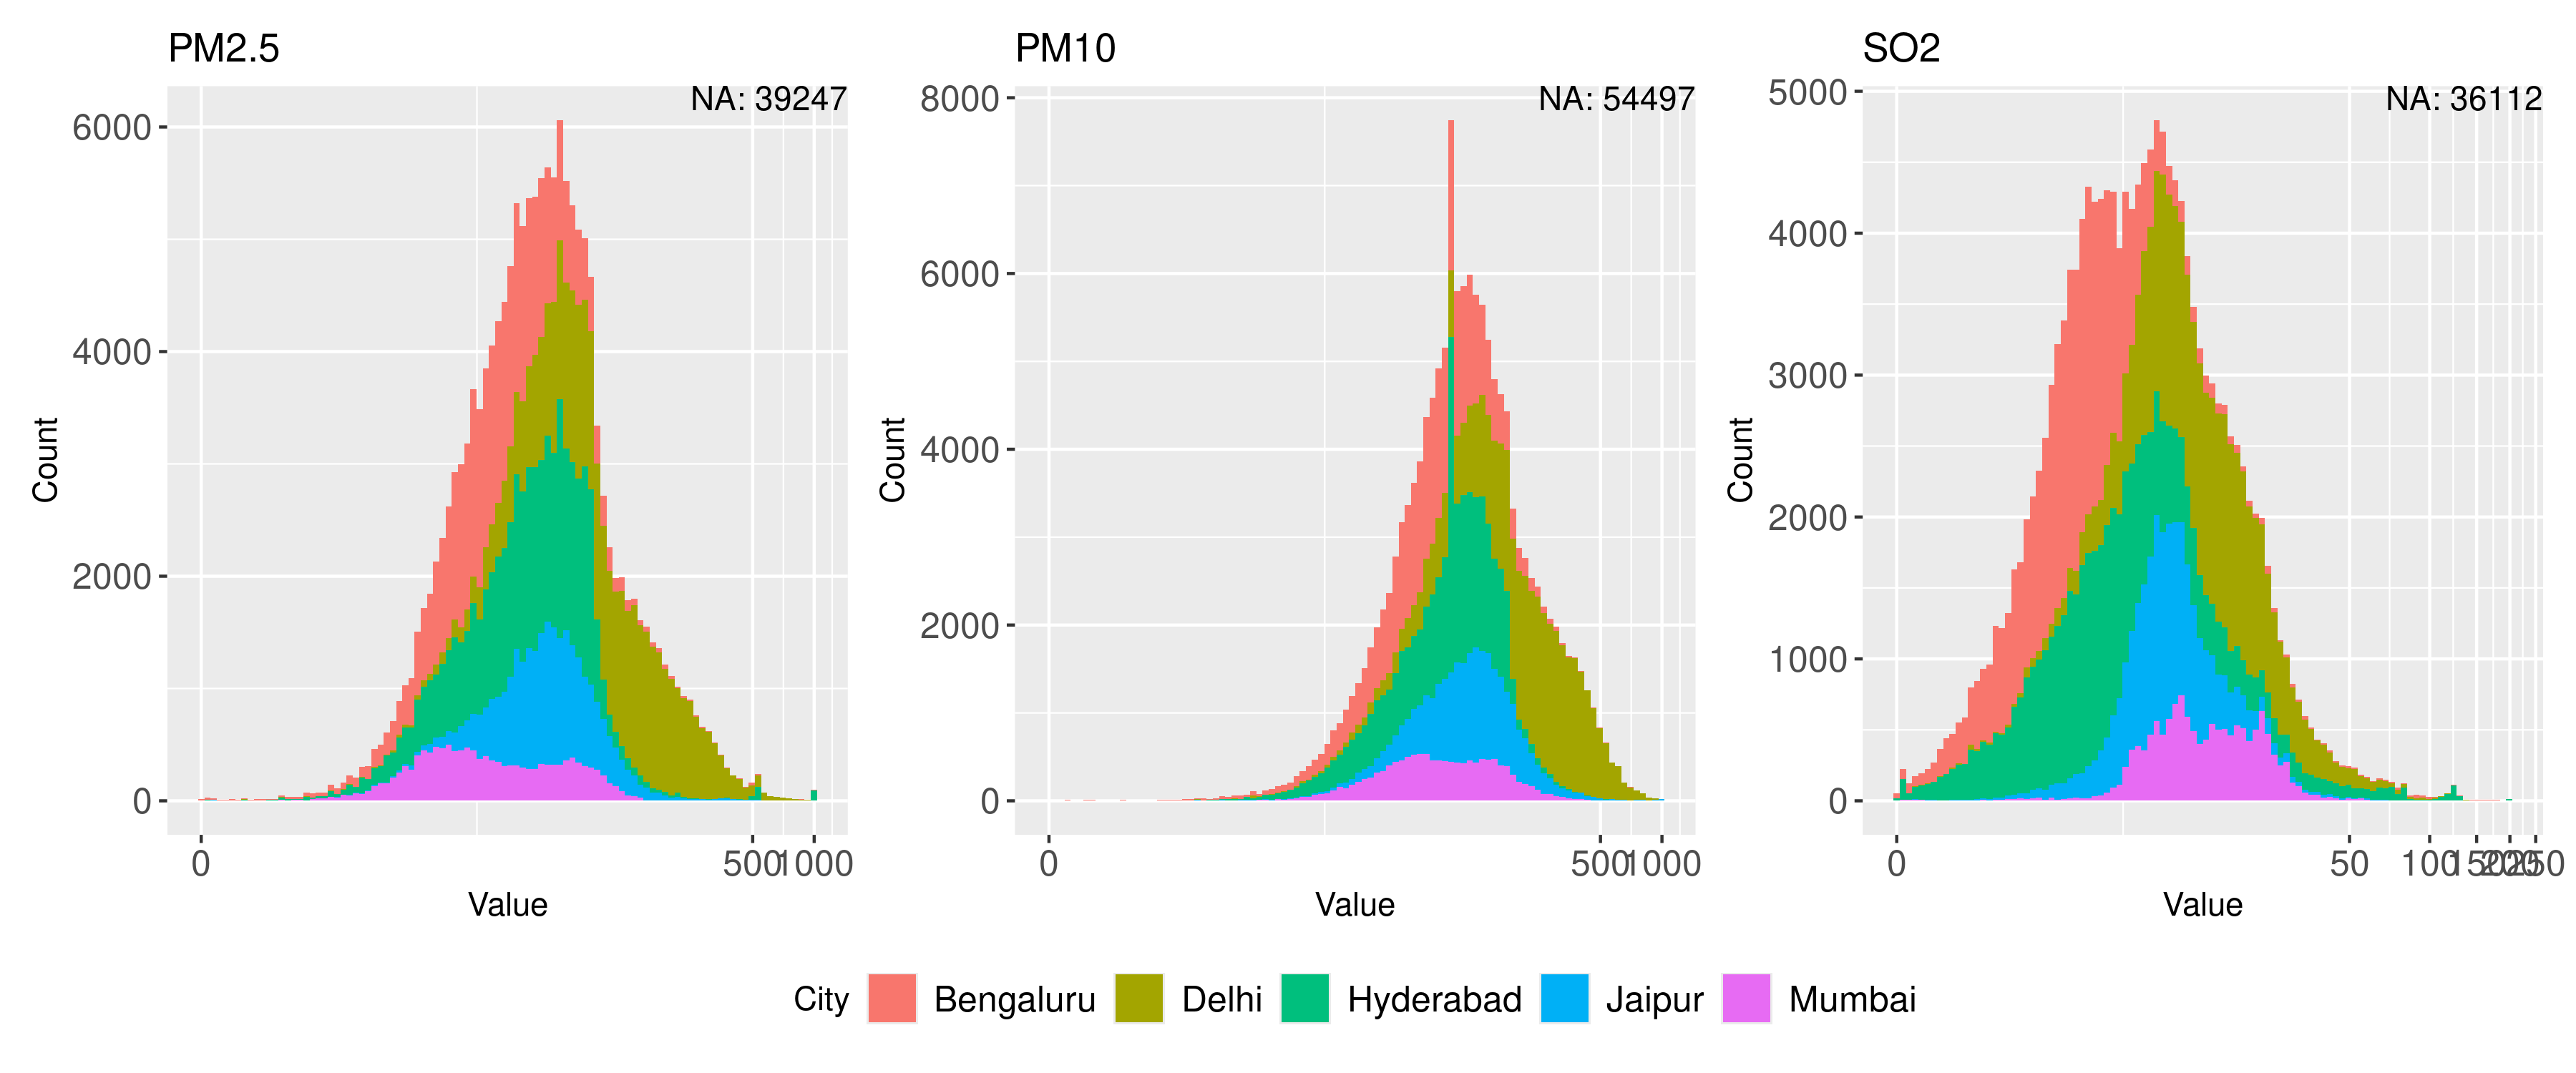
\includegraphics[width=0.7\textwidth]{assets/log-scaled-pollutants.png}
    \end{center}
    \vfill
\end{frame}

\begin{frame}{Feature Engineering}
\begin{itemize}
    \item Temporal Features:
        \begin{itemize}
            \item Hour of day (cyclic encoding)
            \item Day of week
            \item Month of year
        \end{itemize}
    \item Weather-Related Features:
        \begin{itemize}
            \item Wind components (X and Y axes)
            \item 24-hour cumulative precipitation
            \item 24-hour cumulative wind speed
            \item Normalized sunrise times
        \end{itemize}
    \item All continuous features were scaled
\end{itemize}
\end{frame}

\section{Methodology}

\begin{frame}{Model Development}
\begin{itemize}
    \item Independent linear regression models for each:
        \begin{itemize}
            \item City
            \item Response variable
        \end{itemize}
    \item Data splitting:
        \begin{itemize}
            \item Training: 2015-2018
            \item Testing: 2019
        \end{itemize}
    \item Feature selection using VIF analysis
    \item Removed features with VIF > 4:
        \begin{itemize}
            \item minTempC
            \item maxTempC
            \item DewPointC
        \end{itemize}
\end{itemize}
\end{frame}

\begin{frame}{Model Performance by Pollutant}
    \begin{table}
    \centering
    \begin{tabular}{lrrr}
    \hline
    Response & r & R\textsuperscript{2} & RMSE \\
    \hline
    PM2.5 & 0.728 & 0.538 & 0.437 \\
    PM10 & 0.694 & 0.492 & 0.435 \\
    O3 & 0.660 & 0.443 & 0.576 \\
    NOx & 0.430 & 0.214 & 0.604 \\
    NH3 & 0.338 & 0.161 & 0.420 \\
    CO & 0.311 & 0.132 & 0.307 \\
    SO2 & 0.273 & 0.102 & 0.388 \\
    \hline
    \end{tabular}
    \end{table}
    \end{frame}
    
    \begin{frame}{Model Performance by City}
    \begin{table}
    \centering
    \begin{tabular}{lrrr}
    \hline
    City & r & R\textsuperscript{2} & RMSE \\
    \hline
    Delhi & 0.615 & 0.403 & 0.412 \\
    Hyderabad & 0.598 & 0.390 & 0.390 \\
    Bengaluru & 0.427 & 0.246 & 0.481 \\
    Jaipur & 0.411 & 0.198 & 0.472 \\
    Mumbai & 0.061 & 0.007 & 0.649 \\
    \hline
    \end{tabular}
    \end{table}
\end{frame}

\begin{frame}{Key Findings}
\begin{itemize}
    \item Best predictions for:
        \begin{itemize}
            \item PM\textsubscript{2.5} (R\textsuperscript{2} = 0.538)
            \item PM\textsubscript{10} (R\textsuperscript{2} = 0.492)
            \item O\textsubscript{3} (R\textsuperscript{2} = 0.443)
        \end{itemize}
    \item Best performing cities:
        \begin{itemize}
            \item Delhi (R\textsuperscript{2} = 0.403)
            \item Hyderabad (R\textsuperscript{2} = 0.390)
        \end{itemize}
    \item Key predictors:
        \begin{itemize}
            \item Month of year (seasonal patterns)
            \item Humidity (negative correlation)
            \item Wind speed and UV index
        \end{itemize}
\end{itemize}
\end{frame}

\section{Conclusion}

\begin{frame}{Conclusions}
\begin{itemize}
    \item Models show moderate predictive power
    \item Performance varies significantly across:
        \begin{itemize}
            \item Pollutants
            \item Cities
        \end{itemize}
    \item Temporal patterns are strong predictors
    \item Meteorological variables show consistent influence
    \item Linear models capture main relationships
\end{itemize}
\end{frame}

\begin{frame}{Future Work}
\begin{itemize}
    \item Explore more sophisticated approaches:
        \begin{itemize}
            \item Generalized Additive Models (GAMs)
            \item Machine learning techniques
        \end{itemize}
    \item Additional predictors:
        \begin{itemize}
            \item Satellite data
            \item Traffic information
            \item Industrial activity metrics
            \item Special events data
        \end{itemize}
    \item Extend to more cities and longer time periods
\end{itemize}
\end{frame}


\begin{frame}
\begin{center}
\LARGE
\color{mifcolor} Thank you for your attention
\end{center}
\end{frame}

\end{document}